\setchapterpreamble[u]{\margintoc}
\chapter{Statistical Approach to Drop Formation}
\labch{dropstat}

%\input{macros}
\input{nondim}

The destabilization and eventual breakup of ligaments are triggered 
by the growth of undulations that define the initial geometrical shape. 
In the preceding chapter, we have presented our numerical setup pertaining to 
ligaments that are initially at rest, the axisymmetric shapes of which 
are generated in a precisely controllable (and reproducible) manner, 
entailing the superposition of randomly overlapping waves. 
The resulting individual ligaments are characterised primarily 
by the characteristic length scale, aspect ratio and the variance of 
the initial white noise signal used to create the randomly corrugated shape.
Direct numerical simulations (DNS) performed on these ligament shapes 
provide us with important insights, primarily regarding the differences in the 
trajectories of the destabilization and subsequent coalescence dynamics
as a function of the set of initial conditions used. 
In principle we can generate an infinite number of unique initial corrugated shapes 
using our white noise algorithm, each shape characterized by an identical set 
of adimensional parameters ($\textrm{Oh}$, $\varepsilon$, $\Lambda$ and $K$) .
The properties of the drops generated via the ligament breakup 
using the DNS is in strict correspondence to the \textit{exact} initial shape 
of the ligament due to the deterministic nature of the underlying governing equations. 
Therefore, even a slight change in initial conditions lead us to a different collection 
of drops, which may or may not be representative of the total population of drops associated to 
that particular combination of dimensionless parameters. 

In an effort to address this issue, stochasticity is introduced into
the mix by conducting an ensemble of direct numerical simulations of our 
slender corrugated ligaments, where each individual realization corresponds
to a random but unique initial configuration. 
This approach can be viewed as the application of Monte Carlo methods to DNS, 
where uncertainties in the initial conditions are leveraged to provide a statistical 
description of problems which are deterministic in principle. 



\section{Millimeter Scale Ensembles}

We now turn our attention towards slender ligaments whose widths are of the 
order of millimeters, a scale at which a multitude of fragmentation phenomena
\sidenote{Some examples of fragmentation at this length scale involve ligaments
generated by drop splashes on different substrates, secondary atomization of raindrops etc. 
}
take place that are more or less visible to the naked eye.
In particular, for air-water systems (20 degree Celsius) the millimeter length 
scale corresponds to $\textrm{Oh} \sim O(10^{-2})$, where $\textrm{Oh}$ is the Ohnesorge number
based on the characteristic length scale of the ligaments. 
The characterization of our corrugated ligament setup using the set of adimensional
(equation \eqref{base_params}) numbers as discussed in the previous chapter is extended 
to describe our ensemble of ligaments, such that the exact set of parameters
correspond to a unique point in the phase space $\Phi$ of all possible combinations. 
Coalescence that intermittently occurs after the initial breakup phase of 
the thread-like structure not only change the number of drops, but also impacts the 
mean and dispersion of the size distribution due to the increase in the number of drops
significantly larger than the width of the ligament of origin.   
This aspect of temporal dependence of the drop sizes corresponding to a particular ligament ensemble
is taken into account by specifying the time at which the statistics are recorded. 
Thus, our droplet ensembles associated with the millimeter scale ligaments can be uniquely described 
by a combination of the time $T$ and $\Phi_0$, where

\begin{align}
	\Phi_0 \equiv \left( \textrm{Oh}=10^{-2}, K=2\pi, \epsilon=1.0, \Lambda=50 \right). 
\end{align}

The definition of the adimensional groups are identical to that used in the previous chapter.
Statistical descriptions of the drop sizes are commonly carried out using
particular probability density functions (PDF) defined as follows 



\begin{align}
	\text{Gaussian : } \quad P\left( x ; \mu , \sigma \right) &= 
	\frac{1}{\sigma \sqrt{2\pi}} \textrm{exp}\left[-\frac{1}{2}\left(\frac{x - \mu}{\sigma}\right)^2\right] \label{gauss},\\
	\text{Log-Normal : } \quad P\left( x ; \mu , \sigma \right) &= 
	\frac{1}{x \sigma \sqrt{2\pi}} \textrm{exp}\left[-\frac{1}{2}\left(\frac{\log x - \mu}{\sigma}\right)^2\right] \label{log_normal},\\
	\text{Gamma : } \quad P\left( x ; n,k \right) &= 
	\frac{k^{n}}{\Gamma(n)} x^{n-1} \textrm{exp}\left(-k x\right) \label{gamma}, 
\end{align}

where $x$ is the variable (diameter, volume etc) in question. 
The Gamma distribution can be rearranged so that $x$ represents
the variable rescaled by its mean ($n / k$), which becomes 

\begin{align}
	P\left( x ; n \right) = \frac{n^{n}}{\Gamma(n)} x^{n-1} \textrm{exp}\left(-n x\right) . 
\end{align}

The change of variable renders the function dependent solely 
on the parameter $n$, identical to the form first used in \cite{vill_2}
to represent the distribution of the normalized diameter.  
At the large size limit of the distributions, the leading order terms 
scale as $P(x) \sim \textrm{exp}(-x^2)$ for the Gaussian, $P(x) \sim \textrm{exp}(- \log x)$ for 
the Log-Normal and finally $P(x) \sim \textrm{exp}(- x)$ in case of the Gamma function. 
In essence, out of the three density functions, the Guassian predicts the lowest frequency of
rare events (very large drops), the Log-Normal predicts the highest frequency whereas
the Gamma function prediction is somewhere in between the other two. 

\begin{marginfigure}[-1cm]
\centering
\includegraphics{plots/drop_stats/diameter_compute.pdf}
\caption{The shaded area $A$ represented by the dotted and dashed lines
	is used to estimate the diameter of the droplet in question.
	The resulting diameter is computed as $D = \sqrt{4A/\pi}$,
	and the corresponding volume is given by $V = \pi D^3/6$.
	} 
\label{dia_compute}
\end{marginfigure}

Another important aspect to consider is the bin-width of the 
histograms used to construct the probability distributions. 
There are several choices regarding the criteria used to determine the optimal bin-width, 
taking into consideration the size, variability and skewness of the underlying data set. 
In the interest of simplicity, we restrict our focus to histograms with uniform bin-width. 
In order to ascertain the dependence (if any) of the distribution on the number of bins  
(uniform size), we use $4$ different estimators which can be found in the Numpy library \cite{numpy}.
The simplest of the four estimators selects the number 
of bins as the square root of the sample size.
Another estimator is also based solely on the size of the dataset, 
but the number of bins scales as the cube root of the data size.  
A more robust estimator that takes into account the variability in the dataset
is the Freedman Diaconis estimator, in which the bin width is proportional to the 
inter quartile range, and inversely proportional to the cube root of the data size. 
Finally, we also use an improved version of the Sturges estimator, that performs 
well for non-normal datasets due to the fact that it takes into account the skewness. 

In the subsequent sections, we present a statistical picture of the drop sizes generated 
from our ligament ensemble $\Phi_0$, where the sample size is of the order of $64,000$.
The droplet data is primarily recorded on slow time scales, so that the data reflects 
a considerable amount of coalescences after the initial destabilization of the ligaments. 
In order to extract the diameter and volumes of the drops generated in our axisymmetric
simulations, we for the commonly used area based estimation (see Fig. \ref{dia_compute}).


\subsection*{Diameter Distributions}

Figures \ref{t1_dia_bins} and \ref{t2_dia_bins} illustrate the probability distributions
of the normalized droplet diameter corresponding to $T=15$ and $T=30$ respectively. 
The diameters are normalized using the means of the associated samples. 
The bin widths are always based on the properties of the largest sample.
As one can observe, there are fewer drops in all samples at $T=30$ 
compared to the corresponding ones at $T=15$, due to the additional coalescences.  
The drop diameters are found to be more or less symmetrically distributed about the mean,
although there is an small peak at the lower end of the distribution.
The choice of binning criteria does not seem to have any noticeable effect on the 
overall shape of the distribution, regardless of the size of the sample $N$.   
A Gaussian probability density function \eqref{gauss} appears to be a good 
approximation to the underlying distribution.
It is important to note that the Gaussian curve is not fitted to the heights of the 
histogram bins, instead it is plotted on top of the distributions using the mean and 
variance corresponding to the largest sample size, therefore rendering it independent
of the choice of bin-width and free from any additional fitting parameters.  


\begin{figure*}
\centering
\includegraphics{plots/drop_stats/short_time_diameter_bins.pdf}
\caption{Probability distribution functions of the droplet diameter at time $T = 15$. 
	The ensemble is characterized by $\Phi_0 \equiv \left( \textrm{Oh} = 10^{-2}, K = 2\pi , \varepsilon = 1.0 , \Lambda = 50 \right)$. 
The diameters are normalized by the mean of the corresponding sample.  
The distributions are generated using datasets corresponding to four different sample sizes, 
including four different choices of (uniform) bin width. 
The Gaussian functions are characterized by the mean and variance of the original dataset, 
hence they are plotted alongside the histograms instead of being fitted to the bin heights.
	}
\label{t1_dia_bins}
\end{figure*}

% long time scales



\begin{figure*}
\centering
\includegraphics{plots/drop_stats/long_time_diameter_bins.pdf}
\caption{Probability distribution functions of the droplet diameter at time $T = 30$. 
	The ensemble is characterized by $\Phi_0 \equiv \left( \textrm{Oh} = 10^{-2}, K = 2\pi , \varepsilon = 1.0 , \Lambda = 50 \right)$. 
The diameters are normalized by the mean of the corresponding sample.  
The distributions are generated using datasets corresponding to four different sample sizes, 
including four different choices of (uniform) bin width. 
The Gaussian functions are characterized by the mean and variance of the original dataset, 
hence they are plotted alongside the histograms instead of being fitted to the bin heights.
	}
\label{t2_dia_bins}
\end{figure*}

% PDF predictions of data at long times


\begin{figure}
\centering
\includegraphics{plots/drop_stats/long_time_diameter_fits.pdf}
\caption{Probability distribution functions of the droplet diameter at time $T = 30$. 
	The ensemble is characterized by $\Phi_0 \equiv \left( \textrm{Oh} = 10^{-2}, K = 2\pi , \varepsilon = 1.0 , \Lambda = 50 \right)$. 
The diameters are normalized by the mean of the corresponding sample.  
The distribution is generated using 81 bins of uniform size, represented in green.  
The Gaussian and Log-Normal functions are characterized by the mean and variance of the original dataset, 
therefore are plotted alongside the histogram, whereas, the Gamma function is fitted to the bin heights,
with $n= 11.63$ being the value corresponding to the best fit.
	}
\label{t2_dia_fits}
\end{figure}

\begin{figure}
\centering
\includegraphics{plots/drop_stats/long_time_volume_fits.pdf}
\caption{Probability distribution functions of the droplet volume at time $T = 30$. 
	The ensemble is characterized by $\Phi_0 \equiv \left( \textrm{Oh} = 10^{-2}, K = 2\pi , \varepsilon = 1.0 , \Lambda = 50 \right)$. 
The diameters are normalized by the mean of the corresponding sample.  
The distribution is generated using 108 bins of uniform size, represented in green.  
The Gaussian and Log-Normal functions are characterized by the mean and variance of the original dataset, 
therefore are plotted alongside the histogram, whereas, the Gamma function is fitted to the bin heights,
with $n= 1.57$ being the value corresponding to the best fit.
	}
\label{t2_vol_fits}
\end{figure}

% N^{-1/2} scaling of error 

In Fig. \ref{t2_dia_fits}, we present a comparison of the different probability 
density functions applied to the largest ensemble of drops characterized by $\Phi_0$ and $T=30$. 
The Gaussian is found to be the best approximation to the normalized 
diameter distribution, followed by the Gamma and Log-Normal functions.
The Gaussian and Log-Normal curves are generated using the mean and variance 
of the dataset, whereas the free parameter $n$ of the Gamma function is determined
according to the best least-squares fit over the histogram. 
A noteworthy point demonstrated by the inset of Fig. \ref{t2_dia_fits} is that
the error \sidenote{The error is defined as the $L_2$ norm of the differences 
between the bin hights of the sample and the largest sample, where both 
samples have identical bin-width.} scales as $N^{-1/2}$, $N$ being the sample size.
Additionally, the scaling is not sensitive to the choice of bin-width. 
This strongly suggests the absence of any unforeseen correlations between the 
individual realizations (corrugated ligaments) that form the ensemble.


\subsection*{Volume Distributions}

We now shift our attention towards the distribution of droplet volumes. 
Figures \ref{t1_vol_bins} and \ref{t2_vol_bins} show the PDFs 
of the normalized droplet volume corresponding to $T=15$ and $T=30$ respectively. 
The volumes are normalized by the means of the associated samples. 
As in the diameter distributions, the bin widths are always 
based on the properties of the largest sample.
In stark contrast to the case of the diameters, the drop volumes
are found to be heavily skewed towards the smaller sizes.
Similar to the diameter PDFs, the choice of bin-width seems to not have any considerable impact
on the overall shape of the distribution, and is also independent of the sample size.   
In this case though, the single parameter Gamma density function \eqref{gamma} appears to
be the approximation to the volume distribution, with the best fit corresponding to 
values of $n \approx 1.68$ and $n \approx 1.58$ corresponding to $T=15$ and $T=30$ respectively.
There is a slight dependence of the parameter $n$ on the bin-width, which is expected 
as $n$ itself is determined according to the best fit to the histogram in question.

% short time scale 

\begin{figure*}
\centering
\includegraphics{plots/drop_stats/short_time_volume_bins.pdf}
\caption{Probability distribution functions of the droplet volume at time $T = 15$. 
	The ensemble is characterized by $\Phi_0 \equiv \left( \textrm{Oh} = 10^{-2}, K = 2\pi , \varepsilon = 1.0 , \Lambda = 50 \right)$. 
The volumes are normalized by the mean of the corresponding sample.  
The distributions are generated using datasets corresponding to four different sample sizes, 
including four different choices of (uniform) bin width. 
The Gamma functions are characterized by the parameter $n$, the value of which is determined 
by that which provides the best (least-squares) fit to the corresponding bin heights.  
	}
\label{t1_vol_bins}
\end{figure*}

% long time scale

\begin{figure*}
\centering
\includegraphics{plots/drop_stats/long_time_volume_bins.pdf}
\caption{Probability distribution functions of the droplet volume at time $T = 30$. 
	The ensemble is characterized by $\Phi_0 \equiv \left( \textrm{Oh} = 10^{-2}, K = 2\pi , \varepsilon = 1.0 , \Lambda = 50 \right)$. 
The volumes are normalized by the mean of the corresponding sample.  
The distributions are generated using datasets corresponding to four different sample sizes, 
including four different choices of (uniform) bin width. 
The Gamma functions are characterized by the parameter $n$, the value of which is determined 
by that which provides the best (least-squares) fit to the corresponding bin heights.  
	}
\label{t2_vol_bins}
\end{figure*}

Fig. \ref{t2_vol_fits} shows a comparison of the different probability 
density functions applied to the largest ensemble of drops characterized by $\Phi_0$ and $T=30$. 
The Gamma density function seems to be the best representation of the volume distributions.
Considering the Gaussian ($\sim e^{-x^2}$) nature of the diameter ($D$) distributions, a simple variable 
transformation leads us to volume ($D^3$) distributions of the form $\frac{e^{-x^{2/3}}}{x^{2/3}}$, 
which would result in a similar shape as that of the Gamma distribution. 
Similar to the diameter distribution fit, the Gaussian and Log-Normal curves are 
generated using the mean and variance of the dataset, 
whereas the free parameter $n$ of the Gamma function is determined
according to the best least-squares fit over the histogram. 
As seen before, the error (inset of Fig. \ref{t2_vol_fits}) 
scales as $N^{-1/2}$, regardless of the binning criteria used. 

% PDF predictions of data at long times


% N^{-1/2} scaling of error 

\begin{marginfigure}[2cm]
\centering
\includegraphics{plots/drop_stats/amp_long_compare.pdf}
	\caption{The fate of two ligaments whose initial surfaces 
	are created using the same set of random overlapping waves, 
	but differ by the strength of the perturbations.
	The ligament on the left is part of ensemble $\Phi_1$ 
	and the one on the right is part of $\Phi_2$. 
	The droplets enclosed in the boxes (dashed lines)
	are characteristic of the distintegration of weakly perturbed ligaments,
	wherein their sizes are smaller than the typical size at least by a factor of $2$. 
	}
\label{amp_long_comp}
\end{marginfigure}


\subsection*{Influence of Corrugation Amplitude}
As discussed in the previous chapter, the ``smoothness'' of the initial geometrical
shape of the ligament is expected to have a significant influence on the 
destabilization of the liquid thread and the concomitant coalescence dynamics.
In order to ascertain the impact of the strength of the initial perturbations
on the resulting drop size distribution, we conduct simulations of two different 
millimeter scale ensembles $\Phi_1$ and $\Phi_2$, defined below as 

\begin{align}
	\Phi_1 \equiv & \left( \textrm{Oh} = 10^{-2}, K = 2\pi , \varepsilon = 0.4 , \Lambda = 50 \right) ,  \\
	\Phi_2 \equiv & \left( \textrm{Oh} = 10^{-2}, K = 2\pi , \varepsilon = 1.6 , \Lambda = 50 \right) . 
\end{align}

For the case of weakly perturbed ligaments, Fig. \ref{tseries_small} 
demonstrates the temporal evolution of the droplet diameter distributions, 
where the diameter is rescaled by the (mean) width $W$ of the initial ligaments. 
At small time scales, the distribution is bimodal in nature, including a large
number of drops that are smaller than the initial ligament width. 
This may be a consequence of the non-linear effects \cite{sat_1, sat_2} 
that kick in immediately following the initial linear (exponential) growth phase, 
often resulting in the liquid thread disintegrating into a collection of main 
and satellite drops (see Fig. \ref{amp_comp} in the preceding chapter). 
At large times, the peak corresponding to the smaller sizes is considerably diminished, 
whereas the larger size peak develops into more of a ``plateau'' type shape.  
This shift in the distribution in time can be explained by 
successive coalescence, where the smallest drops coalesce with the largest ones. 
By largest drops, we mean the ones situated to the right of the large size peak, 
corresponding to the region of the distribution which eventually 
gives rise to the plateau in the droplet distribution.


Coming to the strongly perturbed ligament shapes, Fig. \ref{tseries_large} illustrates 
the unimodal character of the overall distribution shape.
There seems to be a lack of any significant qualitative change 
when comparing the distributions at small and large time scales. 
The large amplitude perturbations of the ligament surface do not 
allow for any significant amount of liquid rearrangement within the bulk prior 
to disintegration, thus the collection of drops formed immediately following the breakup
of the thread-like structure are quite disperse when with respect to their sizes.
The mean of the distribution displays a slight shift towards the larger sizes, with the passage of time. 
This shift can be explained by the effect of random coalescences amongst droplets corresponding to all sizes.

To summarize, in Fig. \ref{tseries_comp} we present a side-by-side comparison of 
the aforementioned temporal evolutions of the droplet diameter distributions.  
We infer that the primary influence of the corrugation strength 
is that it changes the nature of the resulting distribution from bimodal to unimodal,
as one increases the amplitude of the initial perturbations. 
Although the dynamics of the droplet coalescences (post-breakup) follow different trajectories
in accordance with the corrugation strength (see Fig. \ref{amp_long_comp}), 
the distributions at large times end up looking rather similar.

% temporal variation in drop size PDF's for low and high levels of corrugation

\begin{figure}
\centering
\includegraphics{plots/drop_stats/small_amp.pdf}
\caption{Temporal evolution of the probability distribution functions of the droplet diameter.
	The diameter is rescaled by the initial width $W$ of the ligaments.
	The ensemble is characterized by $\Phi_1 \equiv \left( \textrm{Oh} = 10^{-2}, K = 2\pi 
, \varepsilon = 0.4 , \Lambda = 50 \right)$, thus consisting of \textit{weakly} perturbed 
initial ligaments shapes. 
	}
\label{tseries_small}
\end{figure}

\begin{figure}
\centering
\includegraphics{plots/drop_stats/large_amp.pdf}
\caption{Temporal evolution of the probability distribution functions of the droplet diameter.
	The diameter is rescaled by the initial width $W$ of the ligaments.
	The ensemble is characterized by $\Phi_2 \equiv \left( \textrm{Oh} = 10^{-2}, K = 2\pi 
, \varepsilon = 1.6 , \Lambda = 50 \right)$, thus consisting of \textit{strongly} perturbed 
initial ligaments shapes. 
	}
\label{tseries_large}
\end{figure}

% side by side comparison
% extrapolations of RP etc , limit of volume of largest drop


\begin{figure*}
\centering
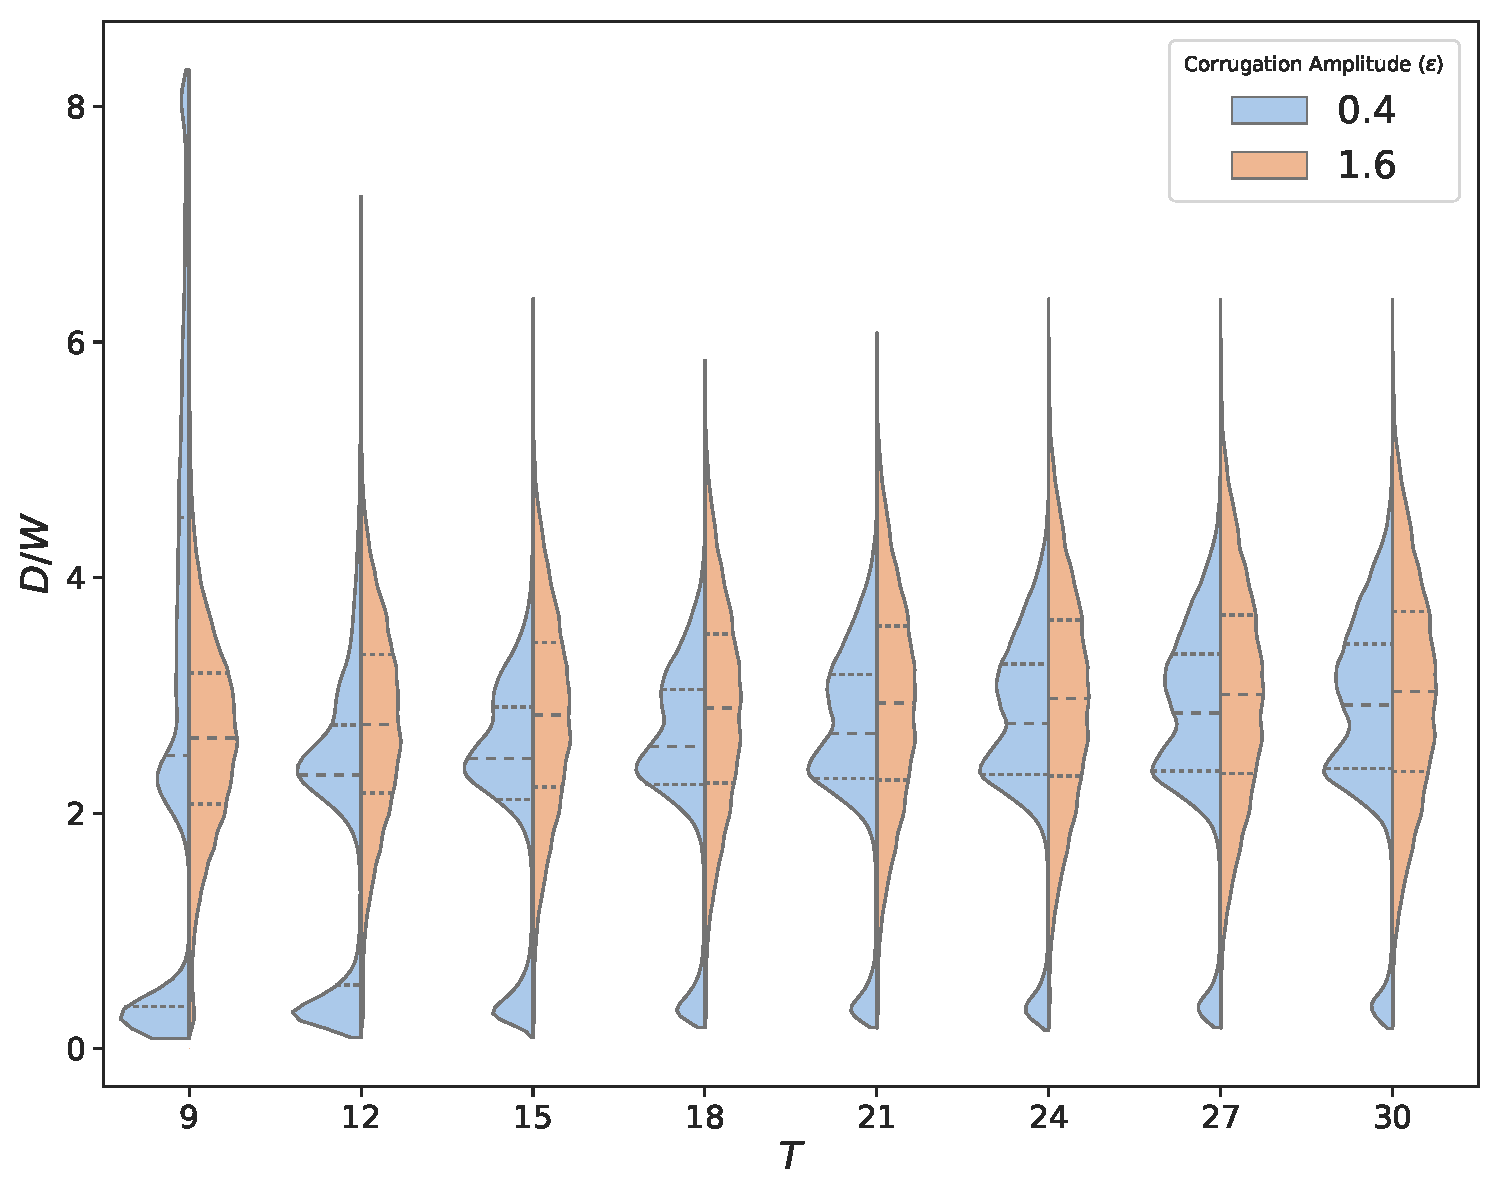
\includegraphics{plots/drop_stats/amp_dist_compare_new.pdf}
\caption{Comparison between the temporal evolution of the probability distribution functions of the
	droplet diameter, corresponding to the strongly ($\varepsilon = 0.4$) and 
	weakly ($\varepsilon = 1.6$) perturbed ligament ensembles. 
	The diameter is rescaled by the width of the initial ligament. 
	The ensembles are characterized by $\Phi_{\{1,2\}} \equiv \left( \textrm{Oh} = 10^{-2}, K = 2\pi 
, \varepsilon = \{0.4,1.6 \} , \Lambda = 50 \right)$. 
The thick dashed lines correspond to the mean of the respective distribution, and the thinner
dashed lines located on both sides of the thicker line corresponding to the respective interquartile ranges. 
	}
\label{tseries_comp}
\end{figure*}


\section{Description of Large Sizes}

The approximately symmetrical diameter distributions that we have seen 
thus far seem to be relatively well described by a Gaussian probability density function. 
We shift our focus to the shape of the distribution towards the right hand 
side of the peak, which represents the large drops emerging from the coalescences.
Although it is quite tempting to conclude that the PDF of the large sizes 
scale as $e^{-x^{2}}$ (where $x = D/\langle D \rangle$), a quantitatively rigourous
procedure is required to ascertain the exact shape in the vicinity of the PDF tail.
In the distributions we have shown thus far, we have not taken into account the 
uncertainties corresponding to the bin heights, which might play a crucial role in determining which among
the candidate scalings (such as $ e^{-x}$, $e^{-x^{2}}$ etc) best describe the rare events. 
In order to compute the error bars associated to the bin heights, we define 
a Bernoulli trial in which a particular drop from the sample size of $N$ either falls into
bin $i$ or not, with an associated probability $p_i$ of falling into that particular bin.
Therefore, $n_i$ drops falling into bin $i$ from a sample of $N$ can be described by a binomial distribution. 
Now, we use a simple model for the bin height uncertainty by setting the length 
of the error bars as the standard deviation 
\sidenote{
The expected value of $n_i$ (where $n_i \sim \mathcal{B}(N,p_i)$) is given by $N p_i$, 
which is equal to the height of bin $i$. 
The corresponding variance of $n_i$ is given by $Np_i(1- p_i)$. 
}
of the corresponding binomially distributed variable. 
Our candidate functions for the large size descriptions are of the form 

\begin{align}
	y = A \cdot \textrm{exp}\left[-n x^m\right] , \quad \text{where} \quad x = D/\langle D \rangle . 
\label{main_func}
\end{align}

The goal is to search for the optimal parameter $m$ such that the function \eqref{main_func} 
is the \textit{best fit} to the bin heights corresponding to the tail region of the distribution.
A non-linear least squares fitting method based on the Levenberg-Marquardt algorithm \sidecite{least_square}
is utilized, through its open-source implementation in the SciPy library \cite{scipy}. 
This fitting routine can find the optimal parameters while taking into account the 
aforementioned uncertainty in the bin heights computed using the binomial variance. 
An important point to note is that even though we can simply find the best fit
to a given set of points, the quality of the fit is also a function
of the number of points used to minimize the least-squares error. 

\begin{marginfigure}[-1cm]
\centering
\includegraphics{plots/drop_stats/window.pdf}
\caption{A representation of the moving window of points which
	is used in our search for the optimal parameters.
	The window starts from the extreme tail end of the 
	distribution, extending towards the peak of the curve
	by including more bin heights on the way. In this 
	particular figure, the window contains $6$ points.
	The minimum size of the window should be greater than
	the number of free parameters in the fitting function.}
\label{window}
\end{marginfigure}


Therefore, we use a moving window of points (see Fig. \ref{window}) and quantify 
the quality of the fit as a function of the number of points used to estimate the optimal parameters.
The ``quality'' of fit is quantified by the standard deviation of the
estimate for ``m", which is returned by the non-linear least-squares fitting algorithm.  
Finally, the value of the optimal parameters that minimize the error 
(standard deviation of parameter estimate) over the different window sizes 
is deemed to be the best fit to our set of bin heights near the tail region.
Additionally, we reframe the fitting problem on logarithmic scales, so 
as to make sure the optimal parameters found are not dependent on the rescaling of the axes. 
Rearranging equation \eqref{main_func} by taking successive logarithms, we obtain 

\begin{align}
Y = m \cdot X + C ,
\label{log_func}
\end{align}

where $Y = \log(-\log y)$ and $X = \log x$, hence transforming it into a linear regression problem.
The overall fitting procedure can be summarized in the following steps : 

\begin{enumerate}
	\item The candidate function is chosen either in the exponential \eqref{main_func}
		or the logarithmic form \eqref{log_func}.
	\item A starting window size (greater than 3 points) is chosen.
	\item The least-squares routine is run using the points falling within the window,
		either by taking into account the uncertainty in the bin heights or not.
	\item An optimal set of parameters ($A$, $n$ and $m$) is found, along with the variance
		of the parameter estimate. 
	\item The above operations are repeated by successively adding more points into the window,
		till the edge of the window reaches the peak of the distribution. 
	\item The parameter $m$ is selected corresponding to the number of points in the window 
		for which the variance in the parameter estimate is minimum. 
\end{enumerate}


\begin{figure}
\centering
	\includegraphics{plots/drop_stats/determine_fit_linear.pdf}
\caption{
	The variation in the optimal parameter $m$ as a 
	function of the number of points in the window (see \ref{window}).
	The least-squares procedure is performed on the 
	candidate function in the exponential \eqref{main_func} form.
	The error bars represent the standard deviation of the 
	parameter estimate obtained from the least-squares routine,
	where the value enclosed in the red box corresponds to the minimum error.
	The figure (a) on top corresponds to the least-squares procedure where the 
	uncertainty in the bin heights is taken into account, whereas the bottom
	figure (b) corresponds to those carried out with zero uncertainty in the underlying distribution. 
	The ensemble is characterized by $\Phi_0 \equiv \left( \textrm{Oh} = 10^{-2}, K = 2\pi 
	, \varepsilon = 1.0 , \Lambda = 50 \right)$ and $T = 30$, 
	thus consisting of \textit{moderately} perturbed initial ligaments shapes. 
	}
\label{determine_linear}
\end{figure}


% without uncertainty

\begin{figure}
\centering
\includegraphics{plots/drop_stats/linear_tail_fit_uncertainty_no.pdf} \\
\includegraphics{plots/drop_stats/linear_zoom_tail_fit_uncertainty_no.pdf} \\ 
\caption{
	The tail of the distribution fitted with the function 
	in the exponential form \eqref{main_func}, using the optimal parameter
	set that corresponds to the lowest standard deviation in the parameter estimate.
	The uncertainty in the bin heights of the underlying distribution is \textit{not}
	taken into account while conducting the least-squares procedure. 
	The bottom figure is a closeup of the region in the vicinity of the tail.
	The ensemble is characterized by $\Phi_0 \equiv \left( \textrm{Oh} = 10^{-2}, K = 2\pi 
	, \varepsilon = 1.0 , \Lambda = 50 \right)$ and $T = 30$, 
	thus consisting of \textit{moderately} perturbed initial ligaments shapes. 
	}
\label{linear_fits_wo}
\end{figure}

% with uncertainty

\begin{figure}
\centering
\includegraphics{plots/drop_stats/linear_tail_fit_uncertainty_yes.pdf} \\
\includegraphics{plots/drop_stats/linear_zoom_tail_fit_uncertainty_yes.pdf} \\ 
\caption{
	The tail of the distribution fitted with the function 
	in the exponential form \eqref{main_func}, using the optimal parameter
	set that corresponds to the lowest standard deviation in the parameter estimate.
	The uncertainty in the bin heights of the underlying distribution \textit{is} 
	taken into account while conducting the least-squares procedure. 
	The bottom figure is a closeup of the region in the vicinity of the tail.
	The ensemble is characterized by $\Phi_0 \equiv \left( \textrm{Oh} = 10^{-2}, K = 2\pi 
	, \varepsilon = 1.0 , \Lambda = 50 \right)$ and $T = 30$, 
	thus consisting of \textit{moderately} perturbed initial ligaments shapes. 
	}
\label{linear_fits_with}
\end{figure}


% log(log) vs log fitting, with and without uncertainty, full distribution and tail zoom  

% methodology to determine best fit

\begin{figure}
\centering
	\includegraphics{plots/drop_stats/determine_fit_log.pdf}
\caption{
	The variation in the optimal parameter $m$ as a 
	function of the number of points in the window (see \ref{window}).
	The least-squares procedure is performed on the 
	candidate function in the logarithmic \eqref{log_func} form.
	The error bars represent the standard deviation of the 
	parameter estimate obtained from the least-squares routine,
	where the value enclosed in the red box corresponds to the minimum error.
	The figure on top (a) corresponds to the least-squares procedure where the 
	uncertainty in the bin heights is taken into account, whereas the bottom 
	figure (b) corresponds to those carried out with zero uncertainty in the underlying distribution. 
	The ensemble is characterized by $\Phi_0 \equiv \left( \textrm{Oh} = 10^{-2}, K = 2\pi 
	, \varepsilon = 1.0 , \Lambda = 50 \right)$ and $T = 30$, 
	thus consisting of \textit{moderately} perturbed initial ligaments shapes. 
	}
\label{determine_log}
\end{figure}

% without uncertainty

\begin{figure}
\centering
\includegraphics{plots/drop_stats/log_tail_fit_uncertainty_no.pdf} \\
\includegraphics{plots/drop_stats/log_zoom_tail_fit_uncertainty_no.pdf} \\ 
\caption{
	The tail of the distribution fitted with the function 
	in the logarithmic form \eqref{log_func}, using the optimal parameter
	set that corresponds to the lowest standard deviation in the parameter estimate.
	The uncertainty in the bin heights of the underlying distribution is \textit{not}
	taken into account while conducting the least-squares procedure. 
	The bottom figure is a closeup of the region in the vicinity of the tail.
	The ensemble is characterized by $\Phi_0 \equiv \left( \textrm{Oh} = 10^{-2}, K = 2\pi 
	, \varepsilon = 1.0 , \Lambda = 50 \right)$ and $T = 30$, 
	thus consisting of \textit{moderately} perturbed initial ligaments shapes. 
	}
\label{log_fits_wo}
\end{figure}


% with uncertainty

\begin{figure}
\centering
\includegraphics{plots/drop_stats/log_tail_fit_uncertainty_yes.pdf} \\
\includegraphics{plots/drop_stats/log_zoom_tail_fit_uncertainty_yes.pdf} \\ 
\caption{
	The tail of the distribution fitted with the function 
	in the logarithmic form \eqref{log_func}, using the optimal parameter
	set that corresponds to the lowest standard deviation in the parameter estimate.
	The uncertainty in the bin heights of the underlying distribution \textit{is} 
	taken into account while conducting the least-squares procedure. 
	The bottom figure is a closeup of the region in the vicinity of the tail.
	The ensemble is characterized by $\Phi_0 \equiv \left( \textrm{Oh} = 10^{-2}, K = 2\pi 
	, \varepsilon = 1.0 , \Lambda = 50 \right)$ and $T = 30$, 
	thus consisting of \textit{moderately} perturbed initial ligaments shapes. 
	}
\label{log_fits_with}
\end{figure}

In figures \ref{determine_linear} and \ref{determine_log} we illustrate the determination
of the optimal parameter set using the moving window of points as descibed previously.
The optimal parameter set corresponding to the lowest standard deviation of the parameter estimate
gives us $m \approx 6$, with the robustness of the result established by the fact that 
it is insensitive to not only the form of the candidate function used, but also does not depend 
on whether the uncertainty in the bin heights are taken into account or not.
This leads us to the rather unusual result that even though the global shape of 
the distribution varies as $e^{-x^2}$, at the limit of large $x$ 
(see figures \ref{linear_fits_wo},\ref{linear_fits_with},\ref{log_fits_wo} and \ref{log_fits_with})
the distribution tail is most accurately described by a function of the form $e^{-x^6}$.
In what follows, we attempt to explain the origin of this scaling
using a random process theory for near-monochromatic waves. 

\section{Theoretical Development}

\newcommand\be{\begin{equation}}
\newcommand\nd{\end{equation}}
\newcommand\ii{{\textrm{i}}}

In the preceding section, we have obtained an exponential scaling for the probability distributions
of drop diameter of the from $\textrm{exp}[-d^6]$, at the limit of large sizes. 
Such a scaling predicts a significantly lower frequency of rare events than all of our candidate 
probability density functions such as the Gaussian, Log-Normal and Gamma. 
In an effort to explain this result, we develop a theoretical model based on the 
linearization of the Navier-Stokes equations for weakly corrugated ligaments, where the ligament destabilizes 
via the growth of perturbations corresponding to a random set of waves, with the assumption
that the wavelengths are more or less normally distributed around the optimal wavelength 
of the Rayleigh-Plateau-Savart instability \cite{rayleigh1879a,plateau1849}.  Note that the mathematical symbols, notations and variable names used in this section are unique to this section only.

In the surface tension dominated regime, it is convenient to rescale all lengths by the
initial unperturbed radius $a$ of the ligaments and times by the capillary time
$\tau = (\rho a^3/\gamma)^{1/2}$ where $\gamma$ is the surface tension.
Our numerical setup is associated to a finite domain such that $0 < x < L$. 
The system is initialized at zero velocity and with a local radius $r(x,0) = 1 + h(x,0)$

\be
h(x,0) = \sum_{n=-N}^{N}  A_n e^{\ii k_n x} ,  \label{p1}
\nd

where $k_n=2\pi n / L$ and $A_n = \overline A_{-n}$. 
The amplitudes $A_n$ are Gaussian independent variables
generated by a pseudo random number generator with identical variance

\be
v_0 = \langle A_n \overline A_n \rangle N ,
\nd

for all $n$. The cutoff frequency defined as $k_N=k_c = 2\pi /L_c$ allows us to obtain a smooth
initial surface profile. The resulting perturbation $h(x,0)$ is also Gaussian with variance $v_0$ 
, which means that there is a finite probability

\be
p_i = \exp[{-1/(2 v_0^2)}] \label{p2}
\nd

that the radius corresponding to the initial condition reaches negative values, 
which is of course unphysical. 
As a result we take care to exclude initializations where at least in one location, 
the local perturbation $h(x,t)$ is close to $-1$ or smaller.

\subsection*{Gaussian random process theory for near-monochromatic waves}

In the regime where $h \ll 1$ the Navier--Stokes equations may be linearized.
After a phase of linear growth, we expect non linear effects to take over 
and the thread to pinch wherever a minimum of radius has developed. 
A simple model accounting for the linear growth is  

\be
h_t = L h , 
\nd

where $L$ is a linear operator on the function $h(x,t)$.
%

\newcommand\hhh{\hat h}

In Fourier space the equation becomes

\be
\hhh_{k,t} = s(k) \hhh_k \label{linth} ,
\nd

where $s(k)$ has a maximum $s_m = s(k_m)$ at the optimal wavelength $k_m = 2\pi/\lambda_m$ of
the Rayleigh-Plateau-Savart instability, with $\lambda_m \sim 9.02 a$. 
As a result one can expand

\be
s(k) \simeq s_m -  C (k - k_m)^2 + \mathcal{O}((k - k_m)^3) , 
\nd

where $s_m$, $C$ and $k_m$ are $\mathcal{O}(1)$ constants in dimensionless variables.
The initial condition is a low-pass filtered noisy shape. We use the theory of
Gaussian processes \sidenote{Refer to \cite{monin1971statistical} Chapter 6 for a good introduction.}.
We represent the initial solution as

\be
h(x,0) = \int_{-\infty}^{\infty}  A(k) e^{\ii k x} {\textrm{d}} k , 
\nd

where $k_M \gg k_m$ is the cutoff defined above in the numerical section. 
The complex amplitudes $A(k)$ form also a Gaussian process \cite{monin1971statistical} with

\be
\langle A(k) \overline A(k^\prime) \rangle = \frac 12 E(k) \delta(k-k^\prime)
\nd

where $E(k)$ is the power spectrum of the initial conditions and
$\langle \cdot \rangle$ is the averaging operator. 
The initial condition is a random function characterised by its variance 
$v_0$, which can be shown using the Wiener-Khinchin theorem to be 

\be
v_0 = \langle h(x,0)^2 \rangle = \int_0^\infty E(k) {\textrm{d}}k . 
\nd

In the numerics we use a low pass filter
\sidenote{Even in the absence of this cutoff the
strong damping of the linear theory would still annihilate the large $k$ modes
thereby giving us identical results.
}
with $E(k)= v_0/(2k_M)$ for $k<k_M$ and $E(k)=0$ otherwise. 
From (\ref{linth}) one has $A(k,t) = A(k) \exp[ s_m t -  C (k - k_m)^2 t]$ and 
at finite time $t$ one has the shape

\be
h(x,t) = \int_{-\infty}^{\infty}  A(k) e^{s_m t -  C (k - k_m)^2 t}  e^{\ii k x} {\textrm{d}} k
\nd

which can be rewritten as 

\be
h(x,t) =  e^{s_m t +\ii k_m x} \int_{-\infty}^{\infty}  B'(\kappa) e^{-  C \kappa^2 t}  e^{\ii \kappa x} {\textrm{d}} \kappa ,
\nd

where $B(\kappa) = A(k_m + \kappa) = \overline A(-k_m -\kappa)$.
The integral on the RHS is a slowly varying modulation of the monochromatic wave $e^{\ii k_m x}$. 
The long lengthscale for this slow variation is $\epsilon^{-1} = (C t)^{1/2}$ and 
the long space variable is $X = \epsilon^{-1} x$, with the corresponding small 
wavenumber $K = \epsilon \kappa$ so that the slow modulation can be rewritten in slow variables as

\be
h(x,t) =   e^{s_m t +\ii k_m x} H(X)  + c.c. \label{slowamp} , 
\nd

where $c.c.$ denotes the complex conjugate and the complex amplitude is

\be
H(X) \simeq \int_{- \infty}^{\infty}  B(K) e^{-K^2}  e^{\ii K X} {\textrm{d}} K \label{saddle} , 
\nd

where $B(K) = B'(\kappa)$. 
The slow modulation can be written as a product of a slowly varying amplitude 
and the exponential of a slow phase $H(X) = \rho(X) \exp [{ \ii \Phi(X) }]$. 
The throats of the  ligament are located at the minima of
$h(x,t)$ that is at places where the total phase
$\phi(x) =  k_m x + \Phi ( X) $ obeys the discrete condition $ \phi(x_n) = 2 n \pi $.
The problem is translationally invariant so without loss of generality the origin can be picked
at a minimum where $\Phi(X) = 0$ so that the next minimum is at $x_1$ such that  $\phi(x_1)= 2 \pi$.
Thus we obtain 

\be
k_m x_1 + \Phi ( \epsilon x_1 ) = 2 \pi , 
\nd

which expresses that $x_1$ is a small perturbation of the optimal Rayleigh-Plateau-Savart wavelength
$x_{R} = 2 \pi / k_m$ and

\be
x_1 = x_R + \Phi(\epsilon x_1)/k_m . 
\nd

Since the variable $X$ is slow at we are looking at small 
distances $X_1 \sim \epsilon x_1$ in the slow variables
one has $\rho(X_1) \simeq \rho_0$ and  $\Phi(X) \simeq \alpha X$ where 
the amplitude $\rho_0$ and the slope $\alpha$ are random
variables. Hence we use the approximation  

\be
x_1 \simeq \lambda_m -  2 \pi \alpha \epsilon  \label{x1a} , 
\nd
(\ref{saddle})

\be
\rho [ 1 + \ii \alpha X] \simeq \int_{-\infty}^{\infty}  B(K) e^{-K^2} ( 1 + \ii K X)  {\textrm{d}} K ,
\nd

and thus

\be
\textrm{Var}(\rho)  \simeq \int_{-\infty}^{\infty} \int_{-\infty}^{\infty}  B(K) B(K') e^{-K^2-K'^2}  {\textrm{d}} K  {\textrm{d}} K'  , 
\nd

and

\be
\textrm{Var}(\rho \alpha) \simeq  \int_{-\infty}^{\infty} \int_{-\infty}^{\infty}  B(K) B(K') e^{-K^2-K'^2}  K 'K {\textrm{d}} K , 
\nd
{\em By the central limit theorem, since $B(K))$ is a Gaussian process, its integrals $\rho$ and $\alpha$ are Gaussian variables.}

To compute their variances we use

\be
\langle B(K) \overline B(K') \rangle = \frac{E(k_m)}{2\epsilon} \delta(K-K') .
\nd

Besides, from (\ref{slowamp}) 

\be
\langle \rho \rangle = \sqrt{v_0/2} . 
\nd

From all the aforementioned relations  

\be
\langle \rho^2 \rangle = \langle \rho \rangle^2 + \langle \rho'^2 \rangle = \frac{\sqrt \pi}{2\sqrt 2} \frac{E(k_m)}{\epsilon} , 
\nd

and

\be
\langle \rho^2 \alpha^2 \rangle = \frac{\sqrt \pi}{8\sqrt 2} \frac{E(k_m)}{\epsilon} . 
\nd

Since

\be
\langle \rho^2 \alpha^2 \rangle =  \langle \rho^2 \rangle \langle \alpha^2 \rangle , 
\nd

one obtains $\textrm{Var}( \alpha ) = \frac 14$
and thus from \eqref{x1a}  $\textrm{Var}(x_1) =\pi^2 \epsilon^2$.
The liquid mass in the interval of lenght $x_1$ will be captured in a breaking droplet
once the nonlinear effects set in, at time $t_{NL}$. This will happen once the
amplitude has reached an order 1 level that is when $t \simeq t_{NL}$ with

\be
t_{NL} \sim \frac 1{2s_m} \ln v_0 .
\nd

Once the breakup happens, the volume of the droplet captured between the throats is
$  V_e = \pi  x_1$ , where the equivalent diameter of the resulting drops is
$\pi d^3/6 =  \pi  x_1$  and $d^3 = 6  x_1$ so that
the variable $d^3$ is Gaussian with standard deviation

\be
\sigma = 6  \pi \left( \frac {2 s_m} {C \ln v_0} \right)^{1/2}
\label{d6_std}
\nd

Using the property 

\be
P_d ( d) {\textrm{d}} d = P_{d^3} (d^3) {\textrm{d}} d^3 ,
\nd

the final droplet size distribution is

\be
  P_{d,G} (d) =  \frac{3 d^2}{\sqrt{2\pi} \sigma} \exp\left[- \frac{(d^3 - d_m^3)^2}{2 \sigma^2}\right] , 
\label{theory_d6}
\nd

where $d_m$ is the equivalent diameter corresponding to the Rayleigh-Plateau wavelength

\be
  \pi  d_m^3/6 \simeq  \pi \lambda_m a^2 , 
\nd

which gives us 

\be
 \frac{d_m}{a} \simeq 3.78  
\nd

\begin{figure*}
\centering
\includegraphics{plots/drop_stats/d6_scaling_compare.pdf}
\caption{Probability distribution functions of the droplet diameter at time $T = 30$. 
	The ensemble is characterized by $\Phi_0 \equiv \left( \textrm{Oh} = 10^{-2}, K = 2\pi , \varepsilon = 1.0 , \Lambda = 50 \right)$. 
The distribution is generated using 81 bins of uniform size, represented in green.  
The Gaussian and Log-Normal functions are characterized by the mean and variance of the original dataset, 
therefore are plotted alongside the histogram, whereas, the Gamma and $d^3$- Gaussian functions are fitted to the bin heights.
	}
\label{d3_gauss}
\end{figure*}


The mechanism described thus far is surface-tension dominated. 
Another mode for breakup arises when the initial distribution reaches 
at some points the nonlinear regime. This occurs randomly along
the ligament length and is thus a Poisson process with probability of 
occurence per unit length

\be
\lambda = \exp[{-1/(2 v_0^2)}]/l_c \label{p3} , 
\nd

where $l_c \sim 1/k_N$ is the correlation length of the initial condition. There is an exponential distribution
of breaking lengths $x_1$ and droplet diameters $d$ with rate $\lambda$ , thus resulting in a distribution of diameters

\be
  P_{d,P} (d) = {3d^2} \lambda e^{-\lambda d^3} \label{PP} .
\nd

For large lengths and small rates $\lambda$, both types of breakup have small probability and the distributions
  combine. A crossover occurs for $d_c$ given by

\be
  {\lambda d_c^3} - \ln \lambda  \sim \frac{(d_c^3 - d_m^3)^2}{2 \sigma^2} , 
\nd

hence

\be
  {\lambda d_c^3} + 1/(2 v_0^2) + \ln l_c \sim \frac{(d_c^3 - d_m^3)^2}{2 \sigma^2} 
\nd 

Defining the length

\be
  \ell = (1/v_0)^{1/3} \sigma^{2/3} \sim   (6  \pi)^{2/3} \left( \frac {2 s_m} {C \ln v_0} \right)^{1/3}  (1/v_0)^{1/3} , 
\nd

in the regime of small $v_0$ one has $\ell \gg d_m$ and thus $d_c \sim \ell$. At $d \gg d_c$ the Poisson distribution
dominates and $P_d(d) \sim P_{d,P}$ . 
For $d \ll d_c$ the $d^3$- Gaussian distribution dominates. 
Therefore, for ligaments corresponding to weakly perturbed initial 
conditions (small corrugation amplitude), a $\textrm{exp}[-d^6]$ 
scaling is expected by virtue of the $d^3$- Gaussian \eqref{theory_d6} predicted by our theory.   
At the time of writing, we do not yet have a large enough ensemble of drops
corresponding to such weakly corrugated ligaments, thus for the time being 
we compare the theoretical prediction to our ensemble of \textit{moderately} 
perturbed ligaments ($\Phi_0$ at $T=30$) as shown in Fig. \ref{d3_gauss}.
The $d^3$- Gaussian does not seem to be the best fit, although  
the mode of the distribution seems to be well approximated by it. 
Revisiting the description of the tail of the drop diameter distributions from 
the previous section, the value of $n$ in the function $y = A\cdot \textrm{exp}[-nx^m]$
is related to the standard deviation of the $d^3$- Gaussian (\eqref{d6_std}). 
We find that the theoretical predictions of $n$ differ significantly 
from what we obtain through our numerical results corresponding to the moderately perturbed ligament ensemble. 
In addition, we do not observe the transition from a $e^{-d^6}$ to a $e^{-d^3}$ scaling 
as predicted in the theory, at least in the few ensembles we have analysed thus far. 

We are currently in the process of applying successive refinements to the 
theoretical development, as well as comparing the dispersion in the droplet sizes 
resulting from the disintegration of large enough ensembles of \textit{weakly} corrugated 
ligaments (the $d^3$- Gaussian prediction is valid only for very small amplitudes).  


